%!TEX root = ../main.tex

\section{Experimental Results}
\label{sec:results}

\subsection{State-Control Results}
Using the formulation of the problem above, \textrm{GPOPS-II} is able to find an optimal solution in a reasonable amount of time (2 min) for a small number of gates (approximately 10).
In \cref{fig:optimized_position}, \cref{fig:optimized_orientation}, we show the optimized states for the 6-gate racetrack of \cref{fig:optimized_trajectory}.

\begin{figure}[htbp]
  \centering
  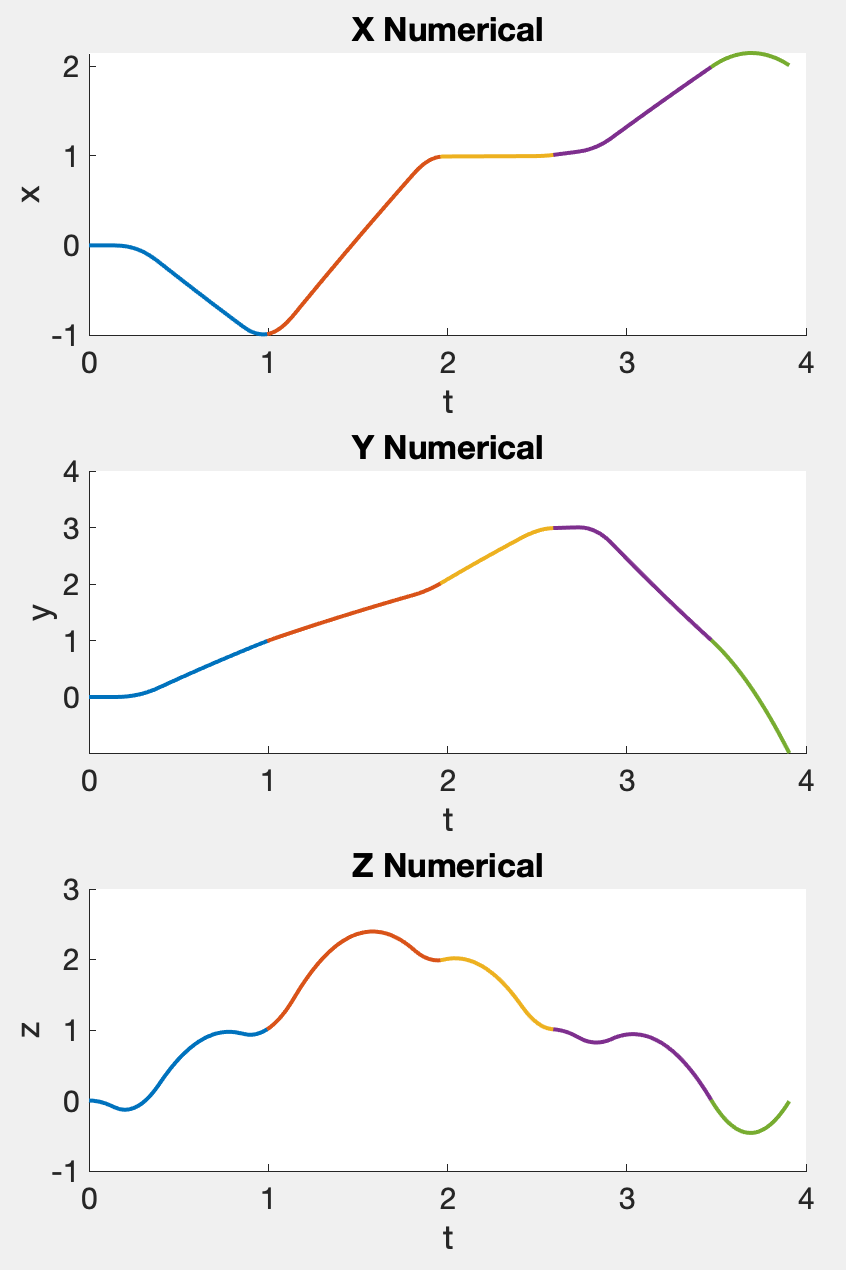
\includegraphics[width=1.0\columnwidth]{img/position.png}
  \caption{Optimized drone positions for the 6-gate environment in \cref{fig:optimized_trajectory}}.
  \label{fig:optimized_position}
\end{figure}

\begin{figure}[htbp]
  \centering
  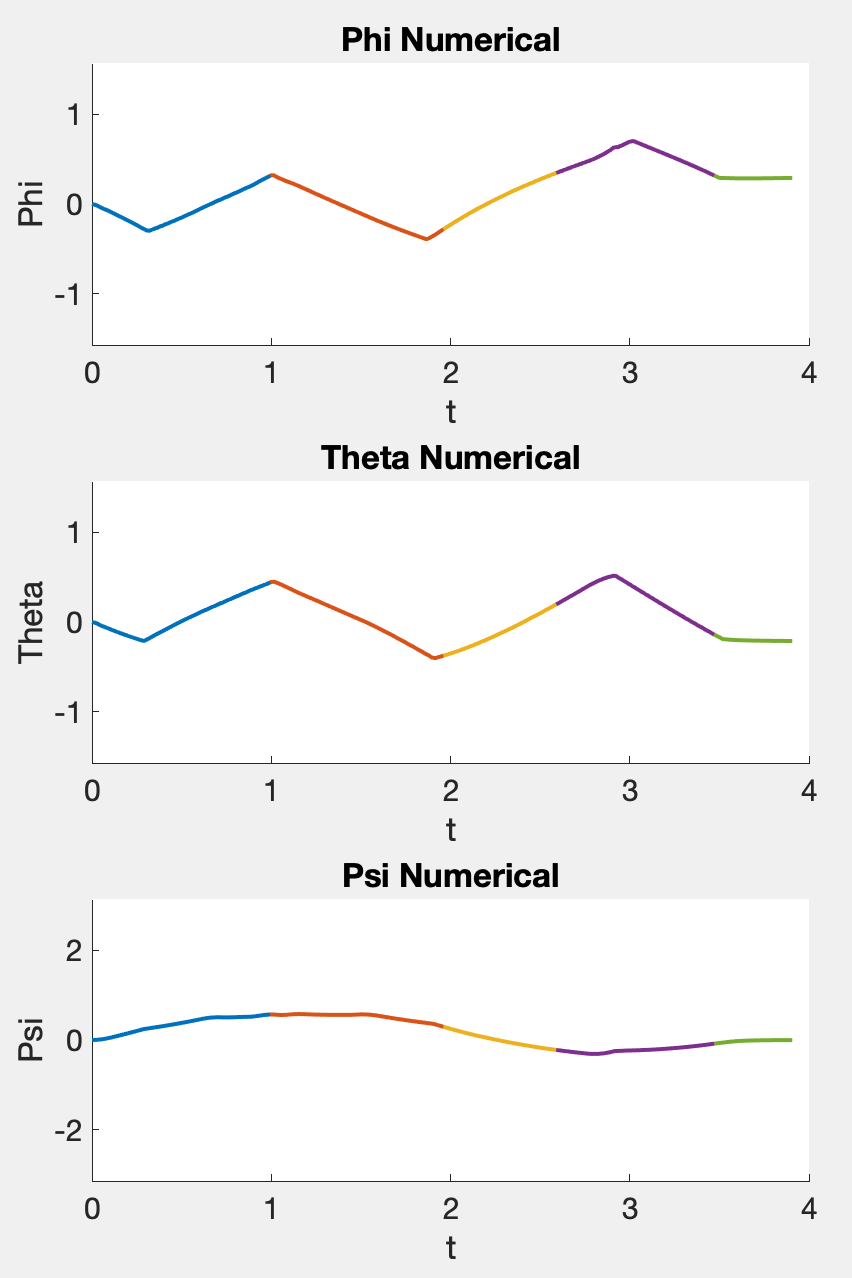
\includegraphics[width=1.0\columnwidth]{img/orientation.png}
  \caption{Optimized drone orientations for the 6-gate environment in \cref{fig:optimized_trajectory}}.
  \label{fig:optimized_orientation}
\end{figure}

\begin{figure}[htbp]
  \centering
  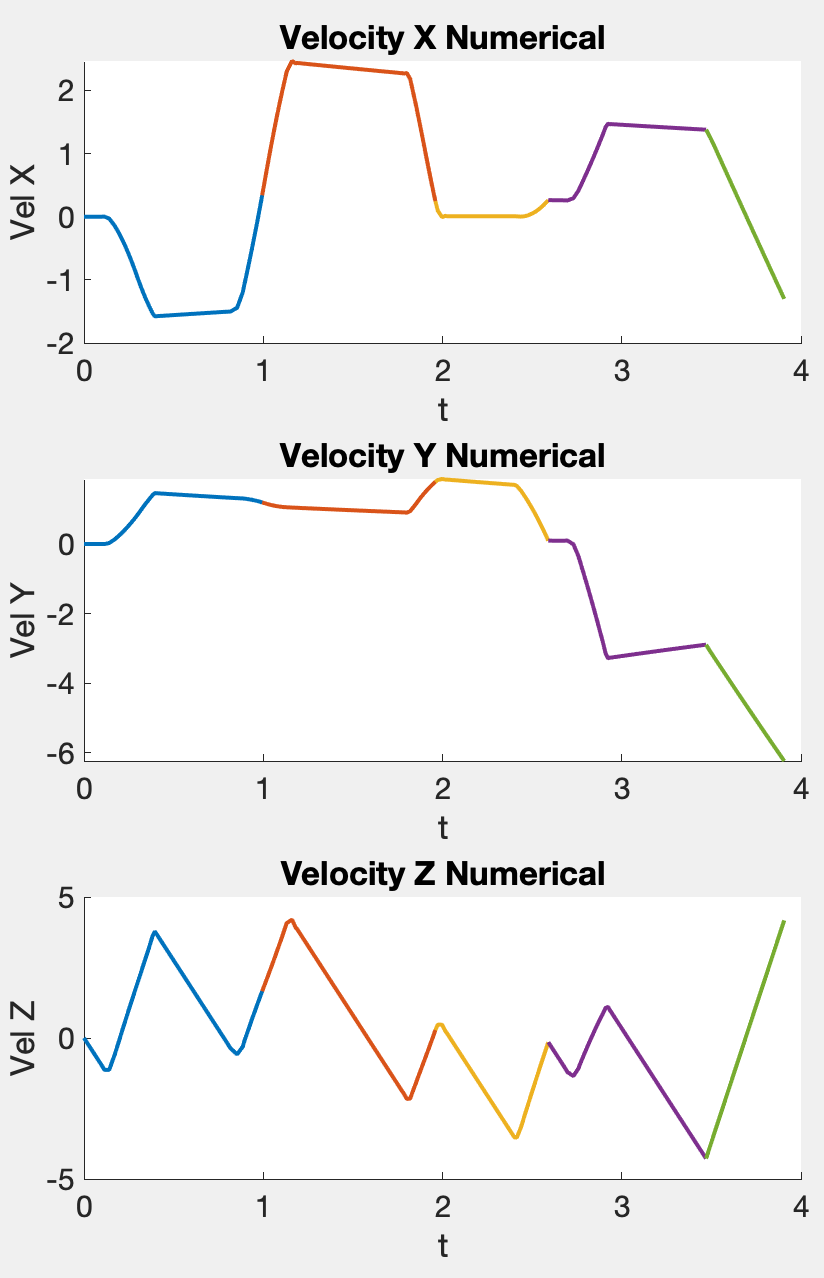
\includegraphics[width=1.0\columnwidth]{img/velocities.png}
  \caption{Optimized drone velocities for the 6-gate environment in \cref{fig:optimized_trajectory}}.
  \label{fig:optimized_velocities}
\end{figure}

\begin{figure}[htbp]
  \centering
  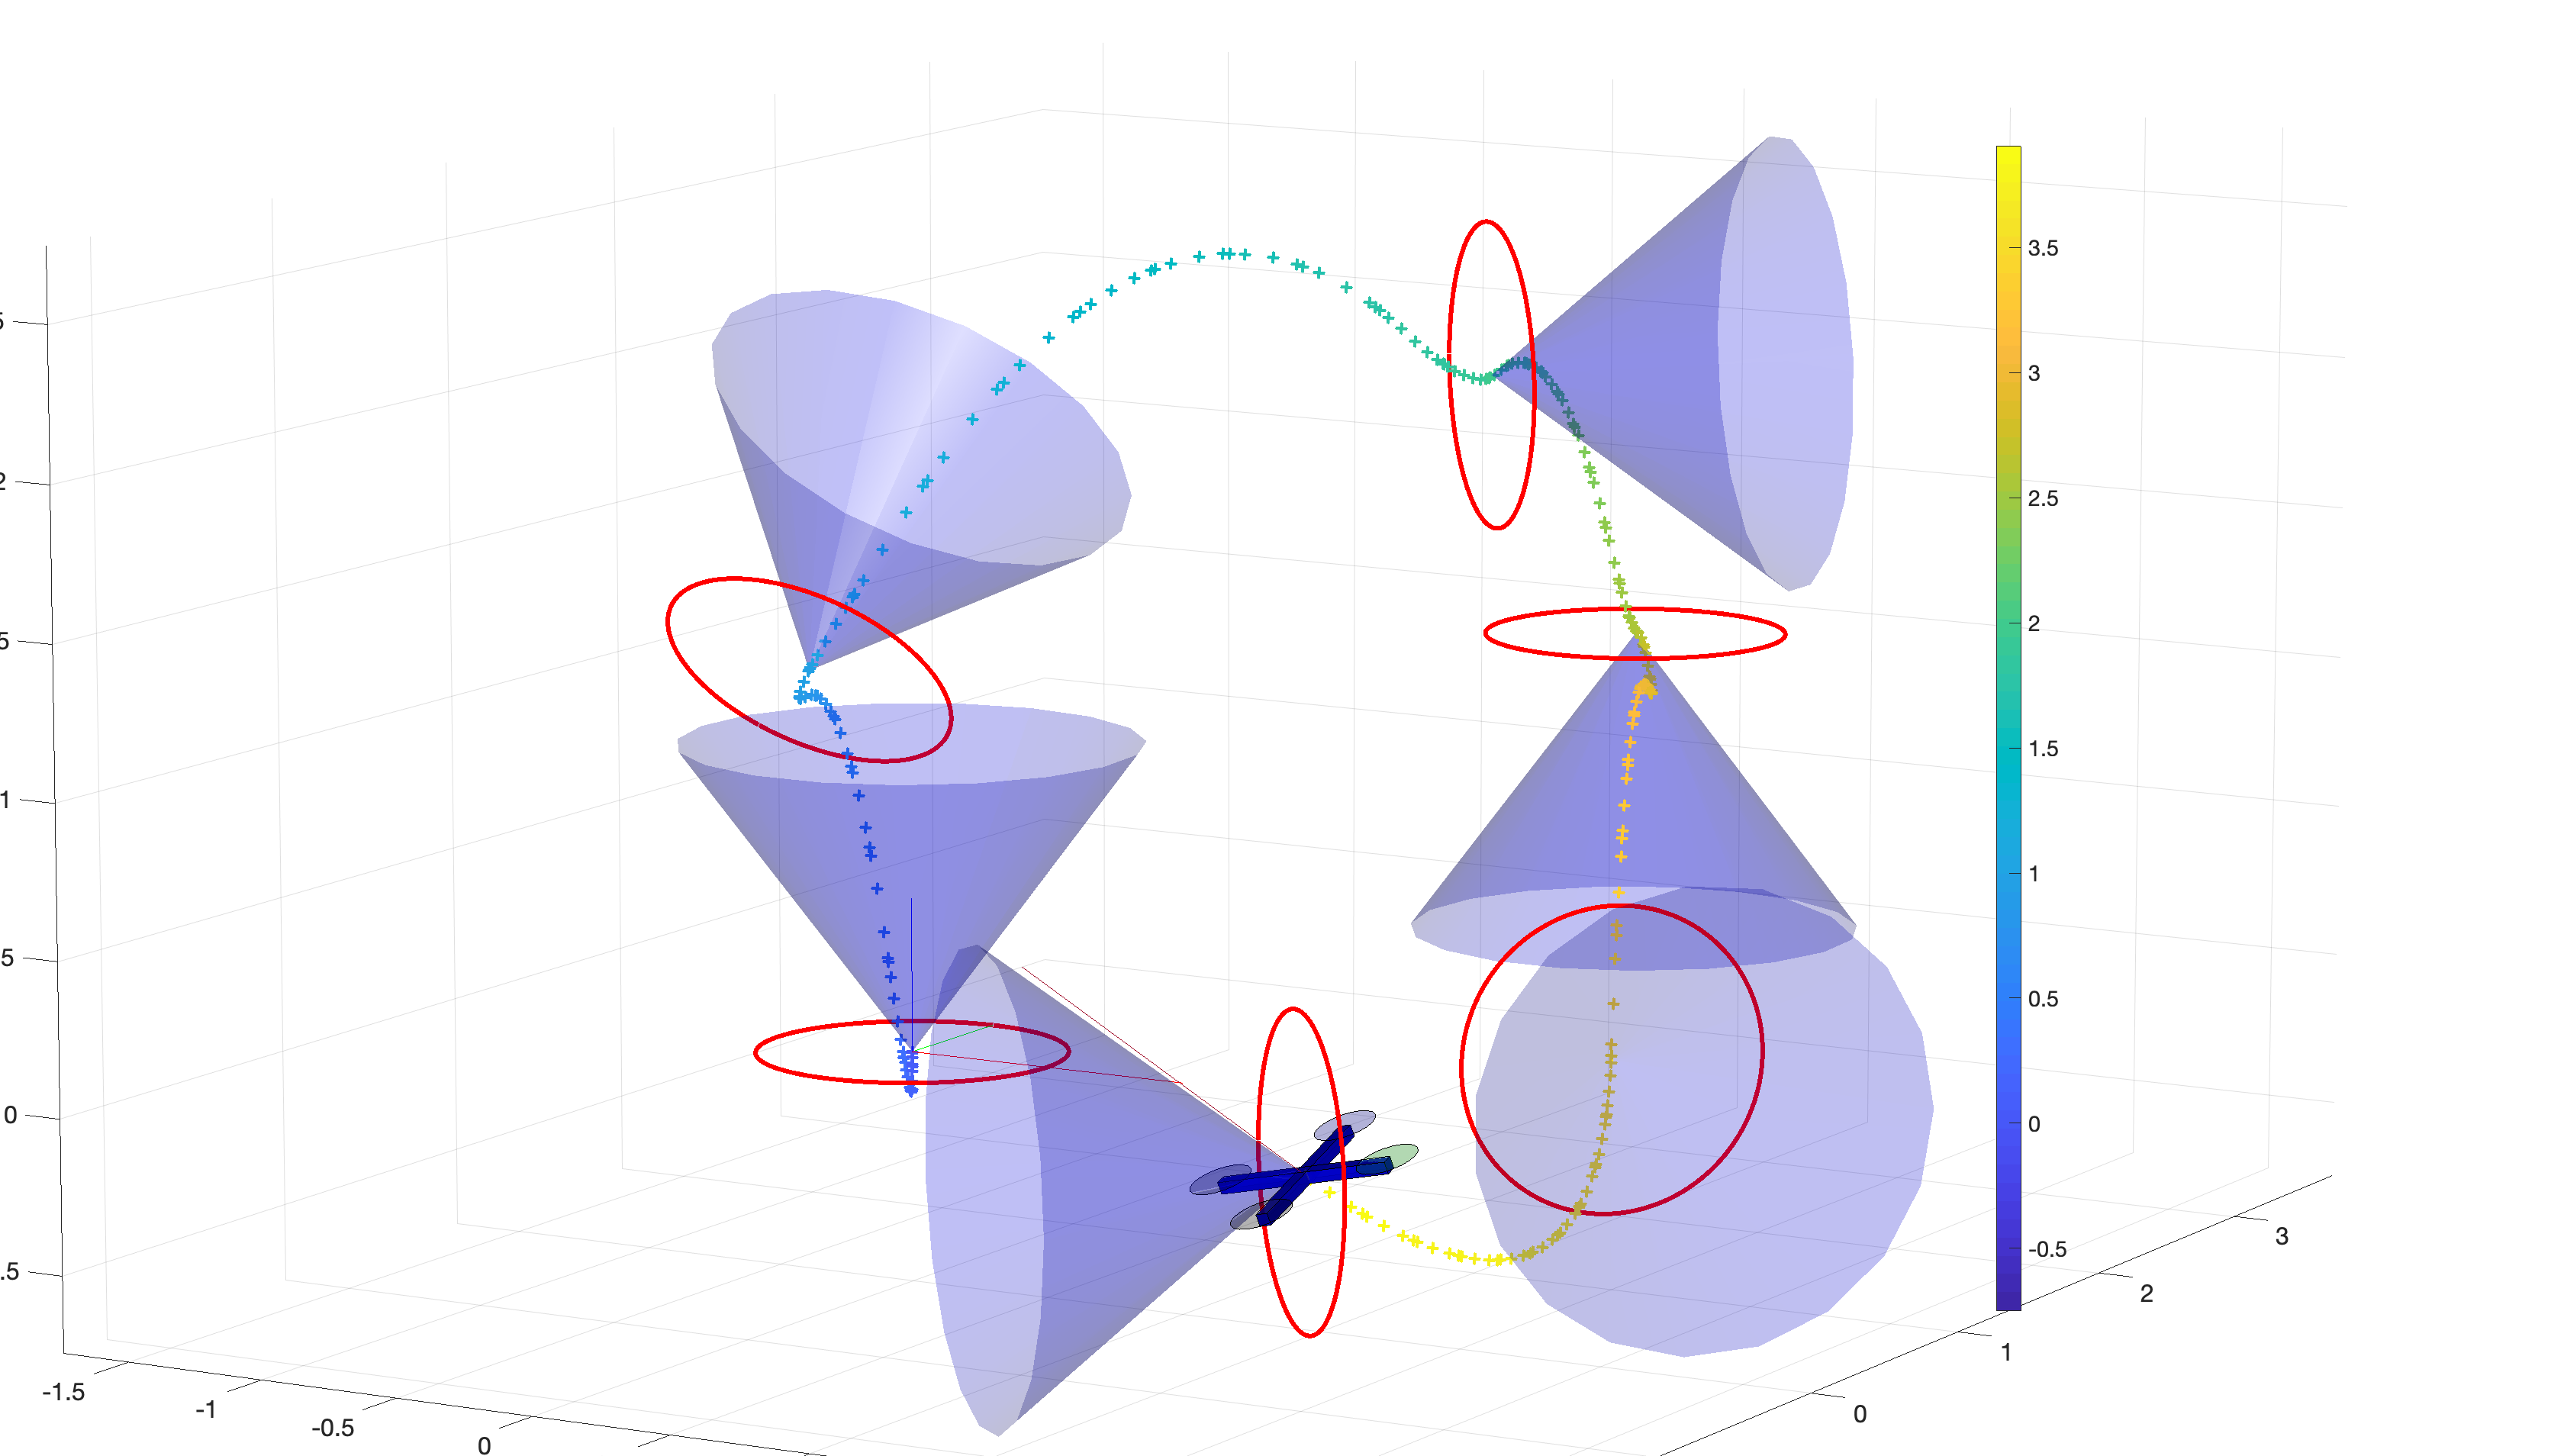
\includegraphics[width=0.8\textwidth, trim=700 0 0 0, clip]{img/DroneRaceTrajectoryOptWCones.png}
  \caption{6-gate drone racetrack with conic velocity constraints to ensure proper traversal of gates.}
  \label{fig:conics}
\end{figure}

\subsection{Modelling Limits}
The way the problem is formulated above does not explicitly encode the fact that the drone must traverse the gate in order to be counted as valid.
Without this explicit constraint, the drone might reach the gate but then depart the same way it arrived to reach the next gate as fast as possible.
Unfortunately, this is not a valid trajectory and therefore we must enforce that the drone traverses the gate fully.
To do so, we make use of event constraints that allow us to constraint the velocity vector of the drone in a cone centered at the origin of the gate and pointing in the same direction as the normal vector of the gate (which we assume is aligned with the sens the gate should be traversed).
In other words, we normalize the velocity vector of the drone, compute the dot product with the normal of the gate and set a threshold on this value, such that the dot product is larger than a positive number less than $1.0$.
In particular, we set this threshold to $0.8$, which leads to satisfactory results.
\Cref{fig:conics} shows the actual cone constraints. The velocity vector is constrained to be inside these cones, at least at the instant of time when the drone is crossing a gate.